\chapter{Learning Regular Expressions}

\label{subsec:regex-def}

\section{Regular Expressions}

Regular expression consist of a finite set of alphabet $\Sigma$ along with three operators $\circ$ (concatenation), $+$ (union), $*$ (kleene star) with the following grammar

$$r:=\varepsilon \mid a\in \Sigma \mid r+r \mid r\circ r \mid r^*$$

The set of all regular expressions over alphabet set $\Sigma$ is referred to as $\mathcal{R}_{\Sigma}$. With slight abuse of notation, another commonly used expression is $r^+$ which refers to the expression $r\circ r^*$. A regular expression can also be represented as a syntax tree where the nodes are labelled by elements from $\Lambda$, where $\Lambda=\Sigma \cup \{\varepsilon, +,\circ,*\}$, that is a combination of alphabets and operators. The alphabets are present only at leaves whereas operators form the internal nodes with the operands being their children.
A syntax DAG can also be created by merging the common subtrees in different branches of a syntax tree. A syntax DAG essentially eliminates redundant subexpressions from a syntax tree. More precisely, the number of nodes in a syntax DAG coincides with the number of subexpressions in the represented expression. The nodes of syntax DAG with $n$ nodes is usually indexed by natural numbers $1,\ldots, n$. The indexing satisfies the property that children of a node are always indexed by numbers smaller than the node itself and only a leaf node can have the index 1. Fig. \ref{fig:syntax_TD} shows what a syntax tree and a syntax DAG looks like. 

\begin{figure}[h!]
\centering
\begin{minipage}{.3\textwidth}
  \centering
\begin{tikzpicture}[-,shorten >=0.5pt,auto, node distance=1.7cm,
                    thick,every state/.style={thick, minimum size=20pt, scale=0.7}]


  \node[state] at (0,0)         (A)  {$+$};
  \node[state] at (-0.75,-1)    (B)  {$\circ$};
  \node[state] at (0.75,-1)     (C)  {$\ast$};
  \node[state] at (-1.5,-2)     (D)  {$a$};
  \node[state] at (0,-2)        (E)  {$b$};
  \node[state] at (0.75,-2)     (F)  {$b$};
  
  \path (A) edge (B)
            edge (C)
        (B) edge (D)
            edge (E)
        (C) edge (F);

\end{tikzpicture}

\end{minipage}%
\begin{minipage}{.3\textwidth}
  \centering
\begin{tikzpicture}[-,shorten >=0.5pt,auto, node distance=1.7cm,
                    thick,every state/.style={thick, minimum size=20pt, scale=0.7}]


  \node[state] at (0,0)         (A)  {$+$};
  \node[state] at (-0.75,-1)    (B)  {$\circ$};
  \node[state] at (0.75,-1)     (C)  {$\ast$};
  \node[state] at (-1.5,-2)     (D)  {$a$};
  \node[state] at (0,-2)        (E)  {$b$};

  
  \path (A) edge (B)
            edge (C)
        (B) edge (D)
            edge (E)
        (C) edge (E);

\end{tikzpicture}

\end{minipage}
\begin{minipage}{.3\textwidth}
  \centering
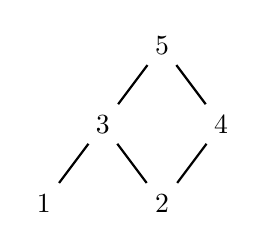
\begin{tikzpicture}[-,shorten >=0.5pt,auto, node distance=1.7cm,
                    thick,every state/.style={thick, minimum size=20pt, scale=0.7}]


  \node at (0,0)         (A)  {$5$};
  \node at (-0.75,-1)    (B)  {$3$};
  \node at (0.75,-1)     (C)  {$4$};
  \node at (-1.5,-2)     (D)  {$1$};
  \node at (0,-2)        (E)  {$2$};

  
  \path (A) edge (B)
            edge (C)
        (B) edge (D)
            edge (E)
        (C) edge (E);

\end{tikzpicture}

\end{minipage}

\end{figure}

\noindent
The semantics of regular expression is generally defined in terms of the language they define:
$$\sema{a}=\{a\};\ \sema{r_1+r_2}=\sema{r_1}\cup\sema{r_2};\ \sema{r_1\circ r_2}=\sema{r_1}\circ \sema{r_2};\ \sema{r^*}=\sema{r}^*$$





Let $w[i,j)$ refer to the subword of $w$ starting from position $i$ and ending at position $j-1$. Also, $w[i,i)=\epsilon$ in this definition. Assume, here that the indexing of word starts from position $0$. 

\begin{definition}{\label{def:match-rel}}

Matching relation $\vdash\subseteq\Sigma^\ast\times \mathcal{R}_\Sigma $ is defined inductively on the structure of a regular expression $r$ in the following manner:
\begin{align*}
&w[i,j)\vdash \epsilon \iff i=j\\
&w[i,j)\vdash a\  \text{where}\ a\in \Sigma \iff w[i,j)=a\\
&w[i,j)\vdash r_1+r_2\ \iff\ w[i,j)\vdash r_1\ \text{or}\ w[i,j)\vdash r_2\\
&w[i,j)\vdash r_1\circ r_2  \iff \exists k\in\mathbb{N}\text{ such that } i\leq k\leq j\text{ and } w[i,k)\vdash r_1 \text{ and } w[k+1,j)\vdash r_2 \\
&w[i,j)\vdash r^* \iff  
\begin{cases}
i=j\text{ or}\\
\exists k\in\mathbb{N} \text{ such that } i< k\leq j \text{ and }w[i,k)\vdash r \text{ and } w[k,j)\vdash r^*
\end{cases}
\end{align*}
\end{definition}

The matching relation $\vdash$ holds true when a word belongs to the language defined by the regular expression. More precisely, we have that ${w[i,j)\vdash r\iff w[i,j)\in\sema{r}}$. This statement can be proved using a simple induction on the structure of $r$. 

Motivated by definition of matching relation, it is possible to design algorithm for checking whether a given word $w$ matches a regular expression $r$, using a \emph{dynamic programming technique}. Let $T_{w}$ be a three dimensional table with $\abs{w}+1$ number of rows and columns both indexed using $0\cdots n$ and the third index is used to denote the subexpression of the expression $r$ for which we are computing the matching relation. The entries of the table have the following meaning.

$$T_w(i,j,r)=1\ \iff w[i,j)\vdash r $$


Given, a regular expression $r$, the table $T_{w}$ is constructed in a iterative manner starting from the portion of the table which refers to the leaf elements of the syntax DAG. These table entries are used for propagating the results to table entries for the internal nodes.\\
\noindent

\begin{itemize}[label=-]
\item For the regular expression $\varepsilon$:\hspace{2pt} $T_{w}(i,j,\varepsilon)=1 \iff i=j$

\item For a leaf node say $a$,\hspace{2pt} $T_{w}(i,j,a)=1 \iff w[i,j)=a$

\item For $+$(union) node, with children $r_1$ and $r_2$:\\$T_w(i,j,r_1+r_2)=1 \text{ if } T_{w}(i,j,r_1)=1 \text{ or } T_w(i,j,r_2)=1$

\item For $\circ$(concat) node, with children $r_1$ and $r_2$:\\$T_w(i,j,r_1\circ r_2)=1 \text{ if } \exists k, i \text{ such that }T_w(i,k,r_1)=1 \text{ and } T_w(k,j,r_2)=1$

\item For $*$(kleene star) node, with a child $r$:\\$T_w(i,j,r^*)=1 \text{ if } \exists k \text{ such that }T_w(i,k,r)=1 \text{ and } T_w(k,j,r^*)=1$
In this case, $T_w$ is filled starting from $(n,n)$th entry up along the columns. 
\end{itemize}
\subsection{The learning problem}
We assume that the data to learn from is given as a pair $\mathcal S = (\mathcal P, \mathcal N)$ consisting of two finite, disjoint sets $\mathcal P, \mathcal N) \subset \Sigma^\ast$ of finite words such that $\mathcal P \cup \mathcal N) \neq \emptyset$.
We call this pair a \emph{sample}.
Moreover, we say that a regular expression $r$ over $\Sigma$ is \emph{consistent} with a sample $\mathcal S = (\mathcal P,\mathcal N)$ if
\begin{enumerate}
	\item $r \vdash u$ for each $u \in \mathcal P$; and
	\item $r \nvdash u$ for each $u \in \mathcal N$.
\end{enumerate}

A possible solution could be to use SAT-solvers to find the regular expression consistent with the given sample. The SAT formula $\varphi_n$ that we feed into the solver has the following structure:

$$\varphi=\varphi^{\text{structure}}_n \wedge  \varphi^{\text{consistency}}_n$$ 
Here, satisfying assignment of $\varphi^{\text{structure}}_n$ provides encoding of a syntax DAG which describes expression of size $n$, while the $\varphi^{\text{consistency}}_n$ checks whether the guessed expression is consistent with the given sample. $\varphi^{\text{structure}}_n$ uses the following variables:

\begin{itemize}[label=$-$]
\item$x_{p,\lambda}$ where $p\in \{1,\cdots, n\}$ and $\lambda\in\Lambda$
\item$l_{p,q}$ where $p\in \{2,\cdots,n\}$ and $q\in\{1,...,p−1\}$
\item$r_{p,q}$ where $p\in \{2,\cdots,n\}$ and $q\in\{1,...,p−1\}$
\end{itemize}
Now, this is how the formula looks like. It is formed by taking conjunction of the following subformulas.

\begin{align}
    [\bigwedge\limits_{1\leq p\leq n} \bigvee\limits_{\lambda \in \Lambda}x_{p,\lambda}]&\wedge[\bigwedge\limits_{1\leq p\leq n}\bigwedge\limits_{\lambda\neq\lambda^{\prime}\in\Lambda}\neg x_{p,\lambda}\vee \neg x_{p,\lambda^{\prime}}]\label{eq:sat1}\\
    [\bigwedge\limits_{2\leq p\leq n} \bigvee\limits_{1\leq q\leq p}l_{p,q}]&\wedge[\bigwedge\limits_{2\leq p\leq n}\bigwedge\limits_{1\leq q\leq q^{\prime}\leq n}\neg l_{p,q}\vee \neg l_{p,q^{\prime}}]\label{eq:sat2}\\
        [\bigwedge\limits_{2\leq p\leq n} \bigvee\limits_{1\leq q\leq p}r_{p,q}]&\wedge[\bigwedge\limits_{2\leq p\leq n}\bigwedge\limits_{1\leq q\leq q^{\prime}\leq n}\neg r_{p,q}\vee \neg r_{p,q^{\prime}}]\label{eq:sat3}\\
    x_{1,\epsilon}&\vee \bigvee\limits_{a\in\Sigma} x_{1, a}\label{eq:sat4}
\end{align}
Subformula~\eqref{eq:sat1} says that each node would be uniquely labelled by an element from $\Lambda$. Subformulas~\eqref{eq:sat2} and~\eqref{eq:sat3} say that each node would have a unique left and right child respectively. Last but not the least, Subformula~\eqref{eq:sat4} says that the first node can have only $\epsilon$ or an alphabet.

First let us consider, for each word $w$ in the given sample, a three dimensional table whose entries are basically variables $y^w_{i,j,p}$, where the indices $i$ and $j$ refers to the substring of the word $w$ and $p$ refers to the sub-expression we are looking at. For simplicity, we assume $m=\abs{w}$. Now, $\varphi^w_n$ is a conjunction of the following subformulas:

\begin{align}
\bigwedge\limits_{1\leq p \leq n}x_{p,\varepsilon}&\rightarrow\Big[\bigwedge\limits_{0\leq i\leq j\leq m }y^w_{i,j,p}\leftrightarrow [i=j]\Big]\label{eq:sat5}\\
\bigwedge\limits_{1\leq p \leq n}\bigwedge\limits_{a\in \Sigma}x_{p,a}&\rightarrow\Big[\bigwedge\limits_{0\leq i\leq j\leq m }
\begin{cases}
y^w_{i,j,p}\text{ if }w[i,j)=a\\
\neg y^w_{i,j,p}\text{ if }w[i,j)\neq a
\end{cases}\Big]\label{eq:sat6}\\
\bigwedge\limits_{\substack{1\leq p \leq n \\ 1\leq q, q^{\prime}\leq p}}x_{p,+}\wedge l_{p,q}\wedge r_{p,q^{\prime}}&\rightarrow\Big[\bigwedge\limits_{\substack{0\leq i \leq j \leq m}}\Big[y^w_{i,j,p}\leftrightarrow y^w_{i,j,q}\vee y^w_{i,j,q^{\prime}}\Big]\Big]\label{eq:sat7}\\  
\bigwedge\limits_{\substack{1\leq p \leq n \\ 1\leq q, q^{\prime}\leq p}}x_{p,\circ}\wedge l_{p,q}\wedge r_{p,q^{\prime}}&\rightarrow\Big[\bigwedge\limits_{\substack{0\leq i\leq j \leq m }}\Big[y^w_{i,j,p}\leftrightarrow \bigvee\limits_{i\leq k\leq j}y^w_{i,k,q}\wedge y^w_{k,j,q^{\prime}}\Big]\Big]\label{eq:sat8} \\
\bigwedge\limits_{\substack{1\leq p \leq n \\ 1\leq q, q^{\prime}\leq p}}x_{p,*}\wedge l_{p,q}&\rightarrow\Big[\bigwedge\limits_{\substack{0\leq i \leq j \leq m}}\Big[y^w_{i,j,p}\leftrightarrow [i=j]\vee \bigvee\limits_{i< k\leq j}y^w_{i,k,q}\wedge y^w_{k,j,p}\Big]\Big] \label{eq:sat9}
\end{align}

The idea for each of these subformulas is motivated by the procedure for filling out the table $T_w$, which in turn essentially uses the way the matching relation has been defined. Using the formula $\varphi^w_n$ for various $w$, we construct $\varphi^\text{consistency}_n$ in the following manner.

\begin{align}
\varphi^\text{consistency}_n=\Big[\bigwedge\limits_{w\in \mathcal P} \varphi_n^{w} \wedge y^w_{0,m,n} \Big]\wedge \Big[\bigwedge\limits_{w\in \mathcal N} \varphi_n^{w} \wedge \neg y^w_{0,m,n} \Big]
\end{align}


Given that we have devised SAT formula for this problem, we utilise it to come up with a simple algorithm using SAT-solvers to find out the smallest regular expression consistent with the sample.
\begin{algorithm}
	\KwIn{A sample $\mathcal S$}
	\DontPrintSemicolon

	\BlankLine
	$n \gets 0$\;
	\Repeat {$\varphi_n^\mathcal S$ is satisfiable, say with model $v$}
	{
		$n \gets n+1$\;
		Construct and solve the formula $\varphi_n^\mathcal S$ using a SAT solver
	}
	\BlankLine
	\Return the regular expression $R^v$\;

	\caption{SAT-based learning algorithm for regular expressions} \label{alg:sat-learner}
\end{algorithm}

\subsection{Proof of correctness}
\begin{claim}
Let $\mathcal{S} = (\mathcal{P}, \mathcal{N})$ be a sample, $n \in \mathbb N \setminus \{ 0 \}$, and $\varphi_n^\mathcal S$ be the propositional formula defined above.
Then, the following holds:
\begin{enumerate}
	\item If there exists a regular expression of size $n$, $R^{\mathcal S}$ that is consistent with $\mathcal S$, then the propositional formula $\varphi_n^\mathcal S$ is satisfiable.
	\item If $v \models \varphi_n^\mathcal S$, then $R^{v}$ is a regular expression of size $n$ that is consistent with $\mathcal S$.
\end{enumerate}
\end{claim}
\begin{proof}
    Using the syntax DAG of the expression $R^{\mathcal S}$ which is indexed using $1\cdots n$, we formulate a valuation $v$ for the propositional variables in $\varphi^{\mathcal S}_n$. We use $R_p^{\mathcal S}$ to refer to the regular expression rooted at the $p^{th}$ node.  
    \begin{itemize}[label=$-$]
    \item We set $v(x_{p,\lambda})=1$ iff the $p^{th}$ node is labelled by $\lambda$.   
    \item We set $v(l_{p,q})=1$ iff $q^{th}$ node is the left child of the $p^{th}$ node and similarly,  $v(r_{p,q})=1$  iff $q^{th}$ node is the right child of the $p^{th}$ node.
    \item We set $v(y^w_{i,j,p})=1$ iff $w[i,j)\vdash R_p^{\mathcal S}$ 
    \end{itemize}
Firstly, it is easy to see that $v\models \varphi_n^{\text{structure}}$, since the formulated valuation ensures the uniqueness of the labels of the nodes as well as that of the left and right children. Moreover, $v\models \varphi^w_n$ for $w\in \mathcal{P}\cup \mathcal{N}$, since, the values of the variables
$y^w_{i,j,p}$ correspond exactly to the valuation of each subexpression $R_i^{\mathcal S}$ on the subword $w[i,j)$. Finally, the fact that $R^{\mathcal S}$ is consistent with $\mathcal S$ implies $v\models y^w_{i,j,p}$ for each $w\in \mathcal P$ and $v\models\neg y^{w}_{i,j,p}$ for each $w\in \mathcal N$. Thus, $v\models \varphi^{\mathcal S}_n$, which proves that $\varphi^{\mathcal S}_n$ is satisfiable.
\\

For the second statement, since, $v\models \varphi^S_n$, we have $v\models \varphi^{\text{structure}}_n$ as well. Hence, the valuation of the variables $x_{p,\lambda}$, $l_{p,q}$, and $r_{p,q}$ encode a syntax DAG from which we obtain the regular expression $R^v$. Again here, we consider $R_p^v$ to be the subexpression of $R^v$ rooted at the $p^{th}$ node. Now, it needs to be shown that $R^v$ is indeed consistent with the sample $\mathcal S$. For that we show, ${v(y^w_{i,j,p})=1 \iff w[i,j)\vdash R^v_p}$ for any $i$,$j\in \{0,\cdots, m\}$ where $m=\abs{w}+1$ and $p\in \{0,\cdots, n\}$. This can be done using induction on the structure of $R^v$.

\begin{itemize}[label=$-$]
    \item \textit{Base case $R^v_p=\varepsilon$}: In this case, $v(x_{p,\epsilon})=1$, which leads to the following implications:
    \begin{align*}
    v(y^w_{i,j,p})=1&\iff i=j  &&\text{[Using Subformula~\eqref{eq:sat5}]}\\
                    &\iff w[i,j)\vdash\varepsilon &&\text{[Using Def.~\ref{def:match-rel}]}
    \end{align*}
    \item \textit{Base case $R^v_p=a$}: In this case, $v(x_{p,a})=1$ and this leads to the following implications: 
    \begin{align*}
    v(y^w_{i,j,p})=1 &\iff w[i,j)=a &&\text{[Using Subformula~\eqref{eq:sat6}]}\\
                     &\iff w[i,j)\vdash a&&\text{[Using Def.~\ref{def:match-rel}]}
    \end{align*}
    \item \textit{Case $R^v_p=R^v_q+R^v_{q^{\prime}}$}: In this case, $v(x_{p,+})$, $v(l_{p,q})$, $v(r_{p,q^{\prime}})$ are all set to 1, and this leads to the following implications:
    \begin{align*}
    v(y^w_{i,j,p})=1 &\iff v(y^w_{i,j,q})=1 \text{ or } v(y^w_{i,j,q^{\prime}})=1 &&\text{[Using Subformula~\eqref{eq:sat7}]}\\
    &\iff w[i,j)\vdash R^v_q\text{ or } w[i,j)\vdash R^v_{q^{\prime}}&&\text{[Using ind. hypothesis]}\\
    &\iff w[i,j)\vdash R^v_q+R^v_{q^{\prime}}&&\text{[Using Def.~\ref{def:match-rel}]}
    \end{align*}
    \item \textit{Case $R^v_p=R^v_q\circ R^v_{q^{\prime}}$}: In this case, $v(x_{p,\circ})$, $v(l_{p,q})$, $v(r_{p,q^{\prime}})$ are all set to 1 and this leads to the following implications:
    \begin{align*}
    v(y^w_{i,j,p})=1 &\iff \exists k\in \mathbb{N},\ 1\leq k\leq m, v(y^w_{i,k,q})=1 \text{ and } v(y^w_{k,j,q^{\prime}})=1 &&\text{[Using Subformula~\eqref{eq:sat8}]}\\
    &\iff \exists k\in \mathbb{N},\ 1\leq k\leq m, w[i,k)\vdash R^v_q \text{ and } w[k,j)\vdash R^v_{q^{\prime}}&&\text{[Using ind. hypothesis]}\\
    &\iff w[i,j)\vdash R^v_q\circ R^v_{q^{\prime}}&&\text{[Using Def.~\ref{def:match-rel}]}
    \end{align*}
    \item \textit{Case $R^v_p=(R^v_q)^{*}$}: In this case, $v(x_{p,*})$ and $v(l_{p,q})$ are set to 1 and this leads to the following implications:
     \begin{align*}
    v(y^w_{i,j,p})=1 &\iff 
    \begin{cases} 
    i=j \text{ or}\\ 
    \exists k\in \mathbb N,\ 1\leq k\leq m,\ v(y^w_{i,k,q})=1 \text{ and }v(y^w_{k,j,p})=1
    \end{cases} &&\text{[Using Subformula~\eqref{eq:sat9}]}\\
    &\iff     
    \begin{cases} 
    i=j \text{ or}\\ 
    \exists k\in \mathbb N,\ 1\leq k\leq m,\ w[i,k)\vdash R^v_q \text{ and }w[k,j)\vdash (R^v_{q})^*
    \end{cases}&&\text{[Using ind. hypothesis]}\\
    &\iff w[i,j)\vdash (R^v_q)^*&&\text{[Using Def.~\ref{def:match-rel}]}
    \end{align*}
    
    Here, we assumed that $v(y^w_{k,j,p})=1$ iff $w[k,j)\vdash R^v_{p}$ in the second step, which cannot be deduced from the induction on the structure of $R^v_p$. This we obtained using another level of induction, which is on the length of the subword that matches $R^v_{p}$. More precisely, we induct on $k$ which ranges from $j$ to $i+1$, where by induction hypothesis, it is assumed that 
    $$v(y^w_{k,j,p})=1 \iff w[k,j)\vdash R^v_{p}\quad \forall k,\ i<k\leq j$$
    The base case occurs when $k=j$, and then, we have 
    ${v(y^w_{k,j,p})=1 \iff k=j  \iff w[k,j)\vdash R^v_{p}}$.

    
\end{itemize}

\end{proof}